\documentclass[12pt]{book}

\usepackage{graphicx,color}
\usepackage{amssymb, amsmath, array}
\usepackage{ccicons}
%\usepackage[a4paper,top=3cm,bottom=2cm,left=2cm,right=2cm,marginparwidth=1.2cm]{geometry}
\usepackage[a4paper,top=3cm,bottom=2cm,left=3cm,right=2cm,marginparwidth=1.2cm,twoside]{geometry}
\usepackage{fancyhdr}
\usepackage{tikz}
\usetikzlibrary{shapes.geometric, arrows}
\usepackage{pgfplots}
\usepackage{caption}
\usepackage{xcolor}
\usepackage{paralist}
\usepackage{mdframed}
\usepgfplotslibrary{fillbetween}
\pgfplotsset{compat=1.18}
\usepackage{float}

\tikzstyle{startstop} = [rectangle, rounded corners, minimum width=3cm, minimum height=1cm,text centered, draw=black, fill=red!30]
\tikzstyle{process} = [rectangle, minimum width=3cm, minimum height=1cm, text centered, draw=black, fill=orange!30]
\tikzstyle{arrow} = [thick,->,>=stealth]
\tikzstyle{box} = [rectangle, minimum width=3cm, minimum height=1cm, text centered, draw=black]

\begin{document}

% Example of title page for the projects carried out within the lasec 

% Simply include it in your mastex tex file: 
%        % Example of title page for the projects carried out within the lasec 

% Simply include it in your mastex tex file: 
%        % Example of title page for the projects carried out within the lasec 

% Simply include it in your mastex tex file: 
%        \input{cover}


% Updated March 2006 (SP)




\newcommand{\logouo}[0]{
  \begin{center}
    
\includegraphics[width=7cm]{Otago.eps}
  \end{center}
  \vspace{0.3cm}
  \hrulefill
}
\newcommand{\project}[1]{
  \begin{center}
    \large{#1}
  \end{center}
  \vspace{1cm}
}
\newcommand{\department}[1]{
  \begin{center}
    \large{#1}
  \end{center}
}
\newcommand{\supervisor}[4]{
  \begin{center}
    \begin{normalsize}{
        \bf #1}\\#2\\#3\\#4
    \end{normalsize}
  \end{center}
}
\renewcommand{\author}[1]{
  \begin{center}
    \Large{#1}
  \end{center}
  \vspace{0.5cm}
}
\renewcommand{\title}[1]{
  \vspace{3cm}
  \begin{center}
    \huge{#1}
  \end{center}
  \vspace{1.7cm}
}
\renewcommand{\date}[2]{
  \begin{center}
    \normalsize{#1 #2}
  \end{center}
  \vspace{0.5cm}
}


\thispagestyle{empty}


% begin title page
  \logouo
  
  \title{STAT115 \\
  Tutoring Materials}
  
  \author{}
  \department{Disability Information and Support (DI\&S)}
  
  \date{July}{2025}

  \begin{center}
    \begin{tabular}{cc}
      \begin{tabular}{p{6.0cm}}
        \supervisor{Tutor}{Eden Li (he/him)}{Ph.: +64 27 361 4776}{Email: eden.li@otago.ac.nz}
      \end{tabular}
    \end{tabular}
  \end{center}
 
% end title page




% Updated March 2006 (SP)




\newcommand{\logouo}[0]{
  \begin{center}
    
\includegraphics[width=7cm]{Otago.eps}
  \end{center}
  \vspace{0.3cm}
  \hrulefill
}
\newcommand{\project}[1]{
  \begin{center}
    \large{#1}
  \end{center}
  \vspace{1cm}
}
\newcommand{\department}[1]{
  \begin{center}
    \large{#1}
  \end{center}
}
\newcommand{\supervisor}[4]{
  \begin{center}
    \begin{normalsize}{
        \bf #1}\\#2\\#3\\#4
    \end{normalsize}
  \end{center}
}
\renewcommand{\author}[1]{
  \begin{center}
    \Large{#1}
  \end{center}
  \vspace{0.5cm}
}
\renewcommand{\title}[1]{
  \vspace{3cm}
  \begin{center}
    \huge{#1}
  \end{center}
  \vspace{1.7cm}
}
\renewcommand{\date}[2]{
  \begin{center}
    \normalsize{#1 #2}
  \end{center}
  \vspace{0.5cm}
}


\thispagestyle{empty}


% begin title page
  \logouo
  
  \title{STAT115 \\
  Tutoring Materials}
  
  \author{}
  \department{Disability Information and Support (DI\&S)}
  
  \date{July}{2025}

  \begin{center}
    \begin{tabular}{cc}
      \begin{tabular}{p{6.0cm}}
        \supervisor{Tutor}{Eden Li (he/him)}{Ph.: +64 27 361 4776}{Email: eden.li@otago.ac.nz}
      \end{tabular}
    \end{tabular}
  \end{center}
 
% end title page




% Updated March 2006 (SP)




\newcommand{\logouo}[0]{
  \begin{center}
    
\includegraphics[width=7cm]{Otago.eps}
  \end{center}
  \vspace{0.3cm}
  \hrulefill
}
\newcommand{\project}[1]{
  \begin{center}
    \large{#1}
  \end{center}
  \vspace{1cm}
}
\newcommand{\department}[1]{
  \begin{center}
    \large{#1}
  \end{center}
}
\newcommand{\supervisor}[4]{
  \begin{center}
    \begin{normalsize}{
        \bf #1}\\#2\\#3\\#4
    \end{normalsize}
  \end{center}
}
\renewcommand{\author}[1]{
  \begin{center}
    \Large{#1}
  \end{center}
  \vspace{0.5cm}
}
\renewcommand{\title}[1]{
  \vspace{3cm}
  \begin{center}
    \huge{#1}
  \end{center}
  \vspace{1.7cm}
}
\renewcommand{\date}[2]{
  \begin{center}
    \normalsize{#1 #2}
  \end{center}
  \vspace{0.5cm}
}


\thispagestyle{empty}


% begin title page
  \logouo
  
  \title{STAT115 \\
  Tutoring Materials}
  
  \author{}
  \department{Disability Information and Support (DI\&S)}
  
  \date{July}{2025}

  \begin{center}
    \begin{tabular}{cc}
      \begin{tabular}{p{6.0cm}}
        \supervisor{Tutor}{Eden Li (he/him)}{Ph.: +64 27 361 4776}{Email: eden.li@otago.ac.nz}
      \end{tabular}
    \end{tabular}
  \end{center}
 
% end title page



\begin{center}
	\ccbyncsa
\end{center}

%%%%%%%%%%%%%%%%%%%%%%%%%%%%%%%%%%%%%%
%%%%%%%%%%%%%%%%%%%%%%%%%%%%%%%%%%%%%%
%%%%%%%%%%%%%%%%%%%%%%%%%%%%%%%%%%%%%%
%%%%%%%%%%TERMS%%%%%%%%%%%%%
%%%%%%%%%%%%%%%%%%%%%%%%%%%%%%%%%%%%%%
%%%%%%%%%%%%%%%%%%%%%%%%%%%%%%%%%%%%%%


\newpage
\thispagestyle{empty}
\mbox{}
\newpage

\setcounter{page}{1}

\pagestyle{fancy}
\lhead{STAT110/115 Tutoring Materials}
\rhead{Terms}

\begin{itemize}
  %----------------------------------------------------------
  % Core population–sample concepts
  %----------------------------------------------------------
  \item \textbf{Population}: the entire group we want to learn about.
  \item \textbf{Sample}: the subset of that population we actually observe.
  \item \textbf{Parameter} (population quantity) vs.\ \textbf{Statistic} (sample-based estimate).

  %----------------------------------------------------------
  % Common symbols
  %----------------------------------------------------------
  \item $\mu$ - population mean \newline \quad\; $\sigma$ - population standard deviation \newline \quad\;
        $\pi$ - population proportion.
  \item $\bar{x}$ - sample mean \newline \quad\; $s$ - sample standard deviation \newline \quad\;
        $\hat{p}$ - sample proportion.

  %----------------------------------------------------------
  % Proportion / ratio / rate
  %----------------------------------------------------------
  \item \textbf{Proportion}: fraction of the (sample or population) total in a given category
        ($0 \le \hat{p} \le 1$).
  \item \textbf{Ratio}: numerator and denominator have the \emph{same} units (e.g.\ waist/hip).
  \item \textbf{Rate}: numerator and denominator have \emph{different} units
        (e.g.\ km per hour; cases per 1,000 person-years).

  %----------------------------------------------------------
  % Random variables
  %----------------------------------------------------------
  \item \textbf{Random variable} $X$: an unknown quantity described by a probability distribution.
  \item \textbf{Observed (realised) value} $x$: the concrete outcome recorded in the data.

  %----------------------------------------------------------
  % Variable types
  %----------------------------------------------------------
  \item \textbf{Variable types}
        \begin{itemize}
          \item \textbf{Quantitative}
                \begin{itemize}
                  \item \emph{Continuous}: can take any value on an interval
                        (e.g.\ height, blood pressure).
                  \item \emph{Discrete}: isolated values, usually counts
                        (e.g.\ number of GP visits).
                \end{itemize}
          \item \textbf{Categorical}
                \begin{itemize}
                  \item \emph{Binary / dichotomous}: two categories
                        (e.g.\ pass vs.\ fail).
                  \item \emph{Nominal}: $\ge 2$ unordered categories
                        (e.g.\ blood type A/B/O/AB).
                  \item \emph{Ordinal}: ordered categories
                        (e.g.\ pain score 0–10, Likert scale).
                \end{itemize}
        \end{itemize}

  %----------------------------------------------------------
  % Censored data – will be revisited in survival analysis weeks
  %----------------------------------------------------------
  \item \textbf{Censored data}
        \begin{itemize}
          \item \textbf{Right-censored}: true value is \emph{greater} than a known limit  
                (e.g.\ patient still alive at study end; age $>90$).
          \item \textbf{Left-censored}: true value is \emph{smaller} than a detection limit  
                (e.g.\ viral load $<10$ copies/mL).
          \item \textbf{Interval-censored}: true value lies between two known bounds  
                (e.g.\ infection occurs between two clinic visits two years apart).
        \end{itemize}
\end{itemize}

%%%%%%%%%%%%%%%%%%%%%%%%%%%%%%%%%%%%%%
%%%%%%%% R (quick-reference) %%%%%%%%%
%%%%%%%%%%%%%%%%%%%%%%%%%%%%%%%%%%%%%%

\newpage
\pagestyle{fancy}
\lhead{STAT110/115 Tutoring Materials}
\rhead{R Functions}

\begin{itemize}

% ============================================================
% 0. Getting started & help
% ============================================================
\item \textbf{Getting help \& packages}
  \begin{itemize}
    \item Install once: \texttt{install.packages("tidyverse")}  \hfill\emph{(data wrangling / plots)}
    \item Load every session: \texttt{library(tidyverse)}
    \item Function help: \texttt{?lm}, worked example: \texttt{example(t.test)}
  \end{itemize}

% ============================================================
% 1. Data import & quick exploration
% ============================================================
\item \textbf{Data import \& quick checks}
  \begin{itemize}
    \item CSV: \texttt{df <- read.csv("myfile.csv", stringsAsFactors = FALSE)}
    \item Peek: \texttt{head(df)}, \texttt{str(df)}, \texttt{summary(df)}
    \item Subset rows: \texttt{dplyr::filter(df, Group == "A")}
  \end{itemize}

% ============================================================
% 2. Descriptive statistics
% ============================================================
\item \textbf{Descriptive statistics}
  \begin{itemize}
    \item Centre: \texttt{mean(x)}, \texttt{median(x)}
    \item Spread: \texttt{sd(x)}, \texttt{IQR(x)}, \texttt{var(x)}
    \item Always add \texttt{na.rm = TRUE} if missing values exist
    \item Correlation: \texttt{cor(x, y)} (number) \; | \;
          \texttt{cor.test(x, y)} (CI + $p$)
  \end{itemize}

% ============================================================
% 3. Graphics (base R)
% ============================================================
\item \textbf{Base R graphics}
  \begin{itemize}
    \item Histogram: \texttt{hist(x, breaks = 20, main = "Histogram")}
    \item Scatterplot: \texttt{plot(df$X, df$Y, main = "Scatterplot")}
  \end{itemize}

% ============================================================
% 4. Probability distributions
% ============================================================
\item \textbf{Key distribution helpers}

  \textbf{Normal} $Z\sim N(0,1)$
  \begin{itemize}
    \item Density: \texttt{dnorm(z)}
    \item Tail area: \texttt{pnorm(q)} ($=P(Z\le q)$)
    \item Quantile: \texttt{qnorm(p)}
    \item Random draw: \texttt{rnorm(n)}
  \end{itemize}

  \textbf{$t$-dist} $T_\nu$
  \begin{itemize}
    \item \texttt{dt(x, df)}, \texttt{pt(t, df)}, \texttt{qt(p, df)}, \texttt{rt(n, df)}
  \end{itemize}

  \textbf{Binomial} $X\sim\mathrm{Bin}(n,\pi)$
  \begin{itemize}
    \item Point prob: \texttt{dbinom(x, n, pi)}
    \item Cumulative: \texttt{pbinom(q, n, pi)}
    \item Quantile: \texttt{qbinom(p, n, pi)}
    \item Random draw: \texttt{rbinom(N, n, pi)}
  \end{itemize}

  \textbf{$\chi^2$ \& F}
  \begin{itemize}
    \item $\chi^2$ tail: \texttt{pchisq(q, df, lower.tail = FALSE)}
    \item Critical $\chi^2$: \texttt{qchisq(0.95, df)}
    \item F tail: \texttt{pf(F, df1, df2, lower.tail = FALSE)}
    \item Critical F: \texttt{qf(0.95, df1, df2)}
  \end{itemize}

% ============================================================
% 5. Confidence intervals & t-tests
% ============================================================
\item \textbf{Confidence intervals \& $t$-tests}
  \begin{itemize}
    \item One-sample mean: \texttt{t.test(x, mu = mu0)}
    \item Two independent groups: \texttt{t.test(y ~ g, data = df)}  
          (\texttt{var.equal = TRUE} for pooled)
    \item Paired: \texttt{t.test(before, after, paired = TRUE)}
    \item Exact one-prop CI / test: \texttt{binom.test(x, n)}
  \end{itemize}

% ============================================================
% 6. Tables & tests for proportions
% ============================================================
\item \textbf{Two-way tables \& $\chi^2$ / Fisher}
  \begin{itemize}
    \item Build: \texttt{tab <- table(df$A, df$B)}; totals: \texttt{addmargins(tab)}
    \item $\chi^2$ test: \texttt{chisq.test(tab)}
    \item Small expected counts? use \texttt{fisher.test(tab)}
  \end{itemize}
\item \textbf{Proportion tests}
  \begin{itemize}
    \item One / two props (large $n$): \texttt{prop.test(x = c(18,12), n = c(30,30))}
  \end{itemize}

% ============================================================
% 7. Linear models & ANOVA
% ============================================================
\item \textbf{Simple \& multiple linear regression}
  \begin{itemize}
    \item Fit: \texttt{fit <- lm(Y ~ X1 + X2, data = df)}
    \item Inspect: \texttt{summary(fit)}; 95\% CI: \texttt{confint(fit)}
    \item Predict: \texttt{predict(fit, newdata = data.frame(X1 = 10, X2 = 5),
          interval = "confidence")}
  \end{itemize}

\item \textbf{Logistic regression (STAT115 Weeks 10-11)}
  \begin{itemize}
    \item Binary outcome: \texttt{logit <- glm(case ~ age + sex,\; family = binomial,\; data = df)}
    \item Odds ratios: \texttt{exp(coef(logit))}; CI: \texttt{exp(confint(logit))}
  \end{itemize}

\item \textbf{One-way ANOVA \& multiple comparisons}
  \begin{itemize}
    \item Overall model: \texttt{a1 <- aov(y ~ group, data = df)}
    \item Summary table: \texttt{summary(a1)}
    \item Pairwise Tukey: \texttt{TukeyHSD(a1)}  \hfill\emph{(controls family-wise error)}
  \end{itemize}

% ============================================================
% 8. Simulation helpers
% ============================================================
\item \textbf{Simulation snippets}
  \begin{itemize}
    \item Reproducibility: \texttt{set.seed(123)}
    \item 1\,000 $N(0,1)$ draws: \texttt{x <- rnorm(1000)}
    \item Central-limit-theorem demo:  
          \texttt{ybar <- replicate(1e4, mean(rnorm(50)))} \hfill\emph{(hist to visualise)}
  \end{itemize}

% ============================================================
% 9. House-keeping
% ============================================================
\item \textbf{Workspace utilities}
  \begin{itemize}
    \item Clear memory: \texttt{rm(list = ls())}
    \item Save history: \texttt{savehistory("my\_hist.Rhistory")}
  \end{itemize}

\end{itemize}


%%%%%%%%%%%%%%%%%%%%%%%%%%%%%%%%%%%%%%
%%%%%%%%% PROBABILITY (Week 2) %%%%%%%
%%%%%%%%%%%%%%%%%%%%%%%%%%%%%%%%%%%%%%

\newpage
\pagestyle{fancy}
\lhead{STAT110/115 Tutoring Materials}
\rhead{Probability}

\begin{itemize}

% -----------------------------------------------------------
% 0. What do we mean by “probability”?
% -----------------------------------------------------------
\item \textbf{Subjective probability} – a personal degree of belief  
      (e.g.\ “I’m 80 \% sure it will rain tomorrow”).
\item \textbf{Objective / long–run probability} – the proportion of times an event occurs
      in a very large number of identical trials (e.g.\ coin toss heads $\approx 0.5$).

% -----------------------------------------------------------
% 1. Sample space \& events
% -----------------------------------------------------------
\item \textbf{Sample space} $S$ – all possible outcomes of an experiment  
      (fair die: $S=\{1,2,3,4,5,6\}$).
\item \textbf{Event} $A$ – a subset of $S$ (e.g.\ “even number” = $\{2,4,6\}$).

% -----------------------------------------------------------
% 2. Basic rules
% -----------------------------------------------------------
\item \textbf{Complement}:\quad $P(A)+P(\overline{A}) = 1$.
\item \textbf{Addition rule} (two events):\quad
      $P(A\cup B)=P(A)+P(B)-P(A\cap B)$.
\item \textbf{Multiplication rule / conditional prob.}:\quad
      $P(A\cap B)=P(A)\,P(B\,|\,A)$.

% -----------------------------------------------------------
% 3. Independence
% -----------------------------------------------------------
\item \textbf{Independent events} – knowing one tells us nothing about the other.
      Equivalent checks:  
      \[
        P(A\cap B)=P(A)\,P(B)\quad\Longleftrightarrow\quad
        P(B)=P(B\,|\,A)\quad\Longleftrightarrow\quad
        P(A)=P(A\,|\,B).
      \]

% -----------------------------------------------------------
% 4. Diagnostic-test notation (STAT115 focus)
% -----------------------------------------------------------
\begin{itemize}
  \item $A$ = person \emph{has} the disease, $\overline{A}$ = person \emph{does not}.
  \item $B$ = test is \emph{positive}, $\overline{B}$ = test is \emph{negative}.
\end{itemize}

\begin{tabular}{@{}ll@{}}
\textbf{Sensitivity} & $P(B\,|\,A)$          – probability the test detects the disease.\\
\textbf{Specificity} & $P(\overline{B}\,|\,\overline{A})$ – probability a healthy person tests negative.\\
\textbf{False-positive rate} & $1-\text{specificity}=P(B\,|\,\overline{A})$.\\
\textbf{Positive Predictive Value (PPV)} & $P(A\,|\,B)$ – “If the test is positive, how likely is disease?”\\
\textbf{Negative Predictive Value (NPV)} & $P(\overline{A}\,|\,\overline{B})$.\\
\end{tabular}

% -----------------------------------------------------------
% 5. Bayes’ theorem (links PPV/NPV to prevalence)
% -----------------------------------------------------------
\[
  P(A\,|\,B)=\frac{P(B\,|\,A)\,P(A)}{P(B\,|\,A)P(A)+P(B\,|\,\overline{A})P(\overline{A})}.
\]
\emph{Tip:} Low disease prevalence ($\downarrow$) $\Rightarrow$ PPV tends to be low even when sensitivity and specificity are high.

% -----------------------------------------------------------
% 6. Two-by-two table quick check
% -----------------------------------------------------------
\[
\begin{array}{c|cc|c}
           & \text{Disease }A & \text{No disease }\overline{A} & \text{Total} \\ \hline
\text{Test + }B     & a & b & a+b \\
\text{Test – }\overline{B} & c & d & c+d \\ \hline
\text{Total} & a+c & b+d & n
\end{array}
\]
\begin{itemize}
  \item Sensitivity $=a/(a+c)$,\; Specificity $=d/(b+d)$.
  \item PPV $=a/(a+b)$,\; NPV $=d/(c+d)$.
\end{itemize}

\end{itemize}


%%%%%%%%%%%%%%%%%%%%%%%%%%%%%%%%%%%%%%
%%%%%%%%%%%%%%%%%%%%%%%%%%%%%%%%%%%%%%
%%%%%%%%%%%%%%%%%%%%%%%%%%%%%%%%%%%%%%
%%%%%%%%CONTINGENCY TABLE%%%%%%%%%
%%%%%%%%%%%%%%%%%%%%%%%%%%%%%%%%%%%%%%
%%%%%%%%%%%%%%%%%%%%%%%%%%%%%%%%%%%%%%
%%%%%%%%%%%%%%%%%%%%%%%%%%%%%%%%%%%%%%

\newpage

\pagestyle{fancy}
\lhead{STAT110/115 Tutoring Materials}
\rhead{Contingency Table}

\begin{itemize}
\item \textbf{Relative Risk (RR)}: Ratio of two probabilities. RR gives the risk of an outcome relative to "exposure". It is calculated as the ratio of the risk of an outcome for an exposed and an unexposed group. $$RR = \frac{a/(a+b)}{c/(c+d)}$$
Meaning of the RR value: RR = 1 there is no association between outcome and exposure (e.g. rugby position and injury). RR < 1 first row happens less likely than the second row. RR > 1 first row happens more likely than the second row.
\item \textbf{Risk Difference (RD)}: Difference between two probabilities. The RD is given by the difference in the risk for the two groups. $$RD = \frac{a}{a + b} - \frac{c}{c + d}$$
\item \textbf{Odds Ratio (OR)}: Ratio of two odds. The OR compares the odds of an outcome for two groups. Ratio of the odds of the outcome for the exposed group to that for the unexposed group. $$OR = \frac{a/b}{c/d} = \frac{ad}{bc}$$. There is no mathematical distinction between exposure and outcome variables -> makes it particularly useful for quantifying associations between binary variables where there is no "direction" e.g. alcohol consumption (Yes/No) and smoking (Yes/No).
\item \textbf{Confidence Interval for Difference Between Two Proportions}: $$p1 = \frac{a}{r1}$$, $$p2 = \frac{c}{r2}$$, $$(p_1 - p_2) \pm Z_{(1 - \frac{\alpha}{2})} \sqrt{\frac{p_1(1-p_1)}{n_1} + \frac{p_2(1-p_2)}{n_2}}$$

\item \textbf{Steps to Calculate the Confidence Interval for Relative Risk}:
    \begin{itemize}
    \item Get the RR value.
    \item Get the ln(RR).
    \item Calculate the SE of ln(RR) (with formula).
    \item Calculate the CI for ln(RR) (with formula).
    \item Calculate the CI for RR (exp() function).
    \end{itemize}
\item \textbf{Standard error for Confidence interval for relative risk:}$$S_{ln}(RR) = \sqrt{\frac{1}{a} - \frac{1}{r_1} + \frac{1}{c} - \frac{1}{r_2}}$$
\item \textbf{Key formula for Confidence interval for relative risk:}$$\ln(RR) \pm Z_{(1-\frac{\alpha}{2})} \cdot S_{\ln(RR)}$$
\item \textbf{Steps to Calculate the Confidence Interval for Odds Ratio}:
    \begin{itemize}
    \item Get the OR value.
    \item Get the ln(OR).
    \item Calculate the SE of ln(OR) (with formula).
    \item Calculate the CI for ln(OR) (with formula).
    \item Calculate the CI for OR (exp() function).
    \end{itemize}
\item \textbf{Standard error for Confidence interval for Odds Ratio:} $$S_{\ln(OR)} = \sqrt{\frac{1}{a} + \frac{1}{b} + \frac{1}{c} + \frac{1}{d}}$$
\item \textbf{The meaning for range of CI:}
\begin{figure} [H]
\centering
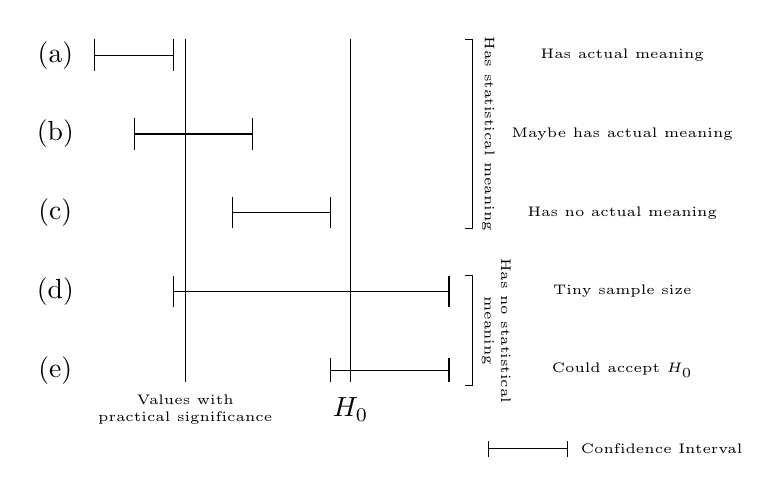
\begin{tikzpicture}
% Horizontal lines with error bars
\draw (0,5) -- (1,5); % Line a
\draw (0, 4.8) -- (0, 5.2); % Error bar for line a
\draw (1, 4.8) -- (1, 5.2); % Error bar for line a

\draw (0.5,4) -- (2,4); % Line b
\draw (0.5, 3.8) -- (0.5, 4.2); % Error bar for line b
\draw (2, 3.8) -- (2, 4.2); % Error bar for line b

\draw (1.75,3) -- (3,3); % Line c
\draw (1.75, 2.8) -- (1.75, 3.2); % Error bar for line c
\draw (3, 2.8) -- (3, 3.2); % Error bar for line c

\draw (1,2) -- (4.5,2); % Line d
\draw (1, 1.8) -- (1, 2.2); % Error bar for line d
\draw (4.5, 1.8) -- (4.5, 2.2); % Error bar for line d

\draw (3,1) -- (4.5,1); % Line e
\draw (3, 0.85) -- (3, 1.15); % Error bar for line e
\draw (4.5, 0.85) -- (4.5, 1.15); % Error bar for line e

\draw (1.15, 0.85) -- (1.15, 5.2); % first bar
\draw (3.25, 0.85) -- (3.25, 5.2); % second bar

% Labels for horizontal lines
\node at (-0.5,5) {(a)};
\node at (-0.5,4) {(b)};
\node at (-0.5,3) {(c)};
\node at (-0.5,2) {(d)};
\node at (-0.5,1) {(e)};

\node [font=\tiny, align=left] at (6.7, 5) {Has actual meaning};
\node [font=\tiny, align=left] at (6.7, 4) {Maybe has actual meaning};
\node [font=\tiny, align=left] at (6.7, 3) {Has no actual meaning};
\node [font=\tiny, align=left] at (6.7, 2) {Tiny sample size};
\node [font=\tiny, align=left] at (6.7, 1) {Could accept $H_0$};

% Vertical text on left
\node[rotate=270, font=\tiny] at (5,4) {Has statistical meaning};

\draw (4.8, 5.2) -- (4.8,2.8);
\draw (4.7, 2.8) -- (4.8,2.8);
\draw (4.7, 5.2) -- (4.8,5.2);

\node[rotate=270, font=\tiny, align=center] at (5.1,1.5) {Has no statistical \\ meaning};
\draw (4.8, 2.2) -- (4.8,0.8);
\draw (4.7, 0.8) -- (4.8,0.8);
\draw (4.7, 2.2) -- (4.8,2.2);


\draw (5,0) -- (6,0); 
\draw (5, -0.1) -- (5, 0.1);
\draw (6, -0.1) -- (6, 0.1); 
\node [font=\tiny, align=left] at (7.2, 0) {Confidence Interval};

% Text below the diagram
\node [font=\tiny, align=center] at (1.15, 0.5) {Values with \\ practical significance};
\node [align=center] at (3.25, 0.5) {$H_0$};

\end{tikzpicture}
\end{figure}
\item \textbf{Risk Difference in Terms of the Number of Cases Per x People}: To get the risk difference in terms of the number of cases per x people, we need to multiply this answer by x. For example, express your answer in terms of the extra number of cases of cancer among 1000 people who eat red or processed meat four or more times per week.  $$\frac{2341}{191678}-\frac{277}{68601}=0.008175$$
To get the risk difference in terms of the number of cases per 1000 people, we need to multiply this answer by 1000. $$RD = \left(\frac{2341}{191678}-\frac{277}{68601}\right)*1000=8.175$$
\end{itemize}


%%%%%%%%%%%%%%%%%%%%%%%%%%%%%%%%%%%%%%
%%%%%%%%%%%% DISTRIBUTIONS %%%%%%%%%%%
%%%%%%%%%%%%%%%%%%%%%%%%%%%%%%%%%%%%%%

\newpage
\pagestyle{fancy}
\lhead{STAT110/115 Tutoring Materials}
\rhead{Distributions}

\begin{itemize}

% ------------------------------------------------------------
% 1. Discrete distributions
% ------------------------------------------------------------
\item \textbf{Bernoulli} ($X\sim\text{Bern}(p)$)\,: one trial, outcome 0/1
      \[
        E(X)=p, \qquad \operatorname{Var}(X)=p(1-p)
      \]

\item \textbf{Binomial} ($X\sim\text{Bin}(n,p)$)\,: $n$ independent Bernoulli trials
      \[
        E(X)=np, \qquad \operatorname{Var}(X)=np(1-p)
      \]
      \[
        P(X=x)=\binom{n}{x}p^{\,x}(1-p)^{\,n-x}
      \]
      \textit{Conditions:} binary outcome, fixed $n$, independent trials, $p$ constant.

% ------------------------------------------------------------
% 2. Continuous distributions
% ------------------------------------------------------------
\item \textbf{Normal family}\,: $X\sim N(\mu,\sigma^2)$  
      \begin{compactitem}
        \item Changing $\mu$ shifts the curve; changing $\sigma$ stretches / shrinks it.
        \item Standard normal: $Z\sim N(0,1)$.
        \item Convert any normal value to a $Z$–score:  
              $Z=(X-\mu)/\sigma$.
      \end{compactitem}

\item \textbf{$t$–distribution}\,: $T_\nu$ has thicker tails than $N(0,1)$;  
      use when population $\sigma$ is unknown and sample size is moderate / small.  
      As $\nu\to\infty$, $T_\nu\to N(0,1)$.

\item \textbf{$\chi^2$ \& $F$}\,: arise from squared $Z$’s and variance ratios;  
      used later for goodness-of-fit, contingency tables, and ANOVA.

% ------------------------------------------------------------
% 3. Sampling distribution of the mean
% ------------------------------------------------------------
\item \textbf{Central Limit Theorem (CLT)}  
      For a simple random sample of size $n$, the \emph{sampling distribution}
      of $\bar{X}$ is \emph{approximately} normal for “large enough” $n$
      (rule-of-thumb $n\ge 30$ if the parent distribution is not too skew).

\item Mean and variance of $\bar{X}$:
      \[
        E(\bar{X})=\mu, \qquad
        \operatorname{Var}(\bar{X})=\frac{\sigma^{2}}{n}, \qquad
        \text{SE}(\bar{X})=\frac{\sigma}{\sqrt{n}}
      \]

\item \textbf{Key take-away}\,: bigger $n\;\Rightarrow\;$ smaller SE $\;\Rightarrow\;$ more precise estimate of $\mu$.

% ------------------------------------------------------------
% 4. Linking histogram ↔ distribution
% ------------------------------------------------------------
\item A \emph{relative-frequency histogram} shows sample data; a \emph{probability
      density function} describes the population.  
      Estimate parameters by $\hat{\mu}=\text{sample mean}$ and
      $\hat{\sigma}=\text{sample sd}$.
      
\item \textbf{Standardising (Z-score)}: $z = \dfrac{X-\mu}{\sigma}$  — converts any $N(\mu,\sigma^2)$ value to the standard normal scale.


\end{itemize}


%%%%%%%%%%%%%%%%%%%%%%%%%%%%%%%%%%%%%%
%%%%%%%% CONFIDENCE INTERVALS %%%%%%%%
%%%%%%%%%%%%%%%%%%%%%%%%%%%%%%%%%%%%%%

\newpage
\pagestyle{fancy}
\lhead{STAT110/115 Tutoring Materials}
\rhead{Confidence Intervals}

\begin{itemize}

% ------------------------------------------------------------
% 1. Concept
% ------------------------------------------------------------
\item \textbf{Goal}: give a plausible range for a population parameter  
      (mean $\mu$, proportion $\pi$, RR, OR, …) based on a random sample.

% ------------------------------------------------------------
% 2. One–sample mean, $\sigma$ known  (rare in real life)
% ------------------------------------------------------------
\item 95\,\% CI when population standard deviation is \emph{known}:
      \[
        \bar{x}\;\pm\;1.96\;
        \frac{\sigma}{\sqrt{n}}
      \]
      \emph{General form:} estimate $\pm$ multiplier $\times$ standard error.

% ------------------------------------------------------------
% 3. One–sample mean, $\sigma$ unknown  (typical)
% ------------------------------------------------------------
\item Replace $\sigma$ by sample $s$ and use the \emph{$t$-distribution}:
      \[
        \bar{x}\;\pm\;t_{1-\alpha/2,\;\nu}\;
        \frac{s}{\sqrt{n}},\qquad
        \nu=n-1
      \]
      • Works if data are (approximately) normal, \textit{or} $n\ge 30$ (CLT).

\item \textbf{99\,\% vs.\ 95\,\%}: larger confidence level $\uparrow$  
      $\Rightarrow$ larger critical value ($1.96\to2.58$)  
      $\Rightarrow$ wider interval.

% ------------------------------------------------------------
% 4. Two independent means
% ------------------------------------------------------------
\item \textbf{Difference of means} ($\mu_1-\mu_2$):
      \[
        (\bar{x}_1-\bar{x}_2)\;\pm\;
        t_{1-\alpha/2,\;\nu}\;
        \sqrt{\frac{s_1^{2}}{n_1}+\frac{s_2^{2}}{n_2}}
      \]
      Use Welch’s $\nu$ (software handles this).

% ------------------------------------------------------------
% 5. Single proportion
% ------------------------------------------------------------
\item Sample proportion: $\hat{p}=x/n$.
      \[
        \hat{p}\;\pm\;1.96\,
        \sqrt{\frac{\hat{p}(1-\hat{p})}{n}}
      \]
      \textit{Conditions}: $n\hat{p}\ge 10$ and $n(1-\hat{p})\ge 10$  
      (ensures normal approximation to binomial).

% ------------------------------------------------------------
% 6. Margin of error \& planning sample size
% ------------------------------------------------------------
\item \textbf{Margin of error (ME)} $=\;$ multiplier $\times$ SE.  
      Desired ME $\Rightarrow$ solve for $n$:
      \[
        n=\left(\frac{z_{1-\alpha/2}\,\sigma}{\text{ME}}\right)^{2},
        \qquad\text{round up}.
      \]

% ------------------------------------------------------------
% 7. Interpretation pitfalls
% ------------------------------------------------------------
\item 95\,\% CI means: “If we \emph{repeated} this study many times,
      95\,\% of the calculated intervals would contain the true parameter.”
      It does \underline{not} say the parameter itself is random.

\item Wider interval $\Leftrightarrow$ more uncertainty  
      (small $n$, large $s$) – always report $n$ alongside the CI.

\end{itemize}

%%%%%%%%%%%%%%%%%%%%%%%%%%%%%%%%%%%%%%
%%%%%%%% HYPOTHESIS TESTING %%%%%%%%%%
%%%%%%%%%%%%%%%%%%%%%%%%%%%%%%%%%%%%%%

\newpage
\pagestyle{fancy}
\lhead{STAT110/115 Tutoring Materials}
\rhead{Hypothesis Testing}

\begin{itemize}
  \setlength{\itemsep}{6pt} %←可自行调小/大

  %----------------------------------------------------------
  % 1. Hypotheses
  %----------------------------------------------------------
  \item \textbf{Null hypothesis} ($H_{0}$): no effect / no difference / no association.
  \item \textbf{Alternative hypothesis} ($H_{A}$): there \emph{is} an effect / difference / association.

  %----------------------------------------------------------
  % 2. Test statistic template
  %----------------------------------------------------------
  \item \textbf{Generic test statistic}
        \[
          \frac{\text{estimate} - \text{null value}}{\text{standard error}}
        \]
        \begin{itemize}
          \setlength{\itemsep}{0pt}
          \item Use $Z$ when $\sigma$ known or $n$ large ($\ge 30$).
          \item Use $t$ (df $=n-1$) when $\sigma$ unknown and sample moderate / small.
        \end{itemize}

  %----------------------------------------------------------
  % 3. $p$-value & rule
  %----------------------------------------------------------
  \item \textbf{$p$-value}: probability of obtaining the test statistic
        (or more extreme) if $H_{0}$ is true.  
        Reject $H_{0}$ when $p<\alpha$ (convention $\alpha=0.05$).

  %----------------------------------------------------------
  % 4. Five-step recipe
  %----------------------------------------------------------
  \item \textbf{Five-step workflow}  
        \begin{enumerate}
          \setlength{\itemsep}{2pt}
          \item State $H_{0}$ and $H_{A}$ (specify one- or two-sided).
          \item Compute test statistic ($Z$ or $t$).
          \item Find $p$-value.
          \item (Optional) Build $(1-\alpha)$ CI — cross-checks decision.
          \item Conclude in plain language.
        \end{enumerate}

  %----------------------------------------------------------
  % 5. Errors & power
  %----------------------------------------------------------
  \item \textbf{Errors \& power}
        \begin{itemize}
          \setlength{\itemsep}{0pt}
          \item Type I ($\alpha$): reject a true $H_{0}$ — false positive.
          \item Type II ($\beta$): fail to reject a false $H_{0}$ — false negative.
          \item Power $=1-\beta$ — boosted by larger $n$ or bigger effect size.
        \end{itemize}

  %----------------------------------------------------------
  % 6. Quick guide table
  %----------------------------------------------------------
  \item \textbf{Common two-sample tests}
        \[
        \begin{array}{lcc}
        \hline
        \text{Scenario} & \text{Test} & \text{R command} \\\hline
        \text{Means, indep.} & t\text{-test (Welch)} & \verb|t.test(y ~ g)|\\
        \text{Means, paired} & \text{Paired }t\text{-test} & \verb|t.test(b, a, paired=TRUE)|\\
        \text{Proportions} & Z\text{-test} & \verb|prop.test(x, n)| \\\hline
        \end{array}
        \]

  %----------------------------------------------------------
  % 7. Chi-square test (categorical × categorical)
  %----------------------------------------------------------
  \item \textbf{$\chi^{2}$ test for independence}
        \begin{enumerate}
          \setlength{\itemsep}{2pt}
          \item $H_{0}$: variables independent; $H_{A}$: associated.
          \item Compute expected counts: $E_{ij}=r_{i}c_{j}/n$.
          \item $\displaystyle\chi^{2}=\sum\frac{(O_{ij}-E_{ij})^{2}}{E_{ij}}$.
          \item df $=(r-1)(c-1)$; get $p$ with \verb|pchisq(..., lower.tail=FALSE)|.
          \item If any $E_{ij}<5$, use \verb|fisher.test| instead.
        \end{enumerate}

  %----------------------------------------------------------
  % 8. CI ↔ hypothesis test
  %----------------------------------------------------------
  \item \textbf{CI vs.\ test linkage:}  
        At the same $\alpha$, a two-sided test and its CI agree:  
        CI excludes null value $\Leftrightarrow$ reject $H_{0}$.
\end{itemize}

%%%%%%%%%%%%%%%%%%%%%%%%%%%%%%%%%%%%%%
%%%%%%%%%%%% REGRESSION %%%%%%%%%%%%%%
%%%%%%%%%%%%%%%%%%%%%%%%%%%%%%%%%%%%%%

\newpage
\graphicspath{{./regressionPic/}}
\pagestyle{fancy}
\lhead{STAT110/115 Tutoring Materials}
\rhead{Regression}

\begin{itemize}
  \setlength{\itemsep}{6pt}  % tighten spacing if desired

% ------------------------------------------------------------
% 0. Overview
% ------------------------------------------------------------
  \item \textbf{Main families of regression}
        \begin{itemize}
          \item \emph{Linear} – outcome \(Y\) \emph{quantitative}.
          \item \emph{Logistic} – outcome binary (0 / 1).
          \item \emph{Cox} – time-to-event in survival analysis (covered later in STAT115).
        \end{itemize}

  \item \textbf{Terminology}
        \begin{itemize}
          \item Explanatory variable \(X\): covariate / predictor / independent var.
          \item Outcome variable \(Y\): response / dependent var.
        \end{itemize}

% ------------------------------------------------------------
% 1. Simple linear regression (SLR)
% ------------------------------------------------------------
  \item \textbf{SLR model}\,: \(Y=\beta_{0}+\beta_{1}x+\varepsilon\)
        \begin{itemize}
          \item \(\mu_{Y|x}=\beta_{0}+\beta_{1}x\) – mean response at \(x\).
          \item \(\beta_{0}\): intercept; \(\beta_{1}\): slope; \(\varepsilon\): random error.
        \end{itemize}

  \item \textbf{Estimated line}\,: \(\hat{y}=\hat{\beta}_{0}+\hat{\beta}_{1}x\),
        where residuals \(\hat{e}_{i}=y_{i}-\hat{y}_{i}\).

  \item \textbf{Least-squares estimates}
        \[
          \hat{\beta}_{1}=\frac{\sum(x_{i}-\bar{x})(y_{i}-\bar{y})}
                               {\sum(x_{i}-\bar{x})^{2}},
          \qquad
          \hat{\beta}_{0}=\bar{y}-\hat{\beta}_{1}\bar{x}.
        \]

  \item \textbf{Key assumptions (“LINE”)}
        \begin{itemize}
          \item \textbf{L}inear relationship between \(\mu_{Y|x}\) and \(x\).
          \item \textbf{I}ndependent observations.
          \item \textbf{N}ormal errors \(\varepsilon\).
          \item \textbf{E}qual error variance (homoscedasticity).
        \end{itemize}

  \item \textbf{Diagnostics}
        \begin{itemize}
          \item Residual plot – check linearity \& equal variance.
          \item Q-Q plot – check normality of residuals.
          \item Leverage / Cook’s distance – spot influential points.
        \end{itemize}

  \item \textbf{Error variance estimate}
        \[
          S^{2}_{e}=\frac{\text{RSS}}{n-2},
          \qquad
          \text{RSS}=\sum\hat{e}_{i}^{2}.
        \]

  \item \textbf{Slope inference}
        \[
          t=\frac{\hat{\beta}_{1}}{\text{SE}(\hat{\beta}_{1})},
          \qquad
          \text{df}=n-2,
          \qquad
          \text{SE}(\hat{\beta}_{1})=
          \frac{S_{e}}{\sqrt{\sum(x_{i}-\bar{x})^{2}}}.
        \]

  \item \textbf{Prediction at \(x_{0}\)}
        \[
          \hat{y}_{0}\pm
          t_{1-\alpha/2,\;n-2}\;
          S_{e}\sqrt{1+\frac{1}{n}+
            \frac{(x_{0}-\bar{x})^{2}}{\sum(x_{i}-\bar{x})^{2}}}.
        \]

% ------------------------------------------------------------
% 2. Correlation summary (optional shortcut)
% ------------------------------------------------------------
  \item \textbf{Correlation coefficient}
        \[
          r=\frac{\sum(x_{i}-\bar{x})(y_{i}-\bar{y})}{
                \sqrt{\sum(x_{i}-\bar{x})^{2}\;
                      \sum(y_{i}-\bar{y})^{2}}}, 
          \qquad -1\le r\le 1.
        \]

  \item \textbf{Coefficient of determination}\,: \(R^{2}=1-\text{RSS}/\text{TSS}\)
        – fraction of variance in \(Y\) explained by the model.

% ------------------------------------------------------------
% 3. Logistic regression (binary outcome) – STAT115 focus
% ------------------------------------------------------------
  \item \textbf{Logistic model}
        \[
          \log\!\bigl(\tfrac{p}{1-p}\bigr)
          =\beta_{0}+\beta_{1}x,
          \qquad
          p=P(Y=1).
        \]

  \item \textbf{Interpretation}\,: one-unit increase in \(x\)
        multiplies the \emph{odds} by \(\exp(\beta_{1})\).

  \item \textbf{Inference on \(\beta_{1}\)}
        \[
          z=\frac{\hat{\beta}_{1}}{\text{SE}(\hat{\beta}_{1})},
          \qquad
          p\text{-value from }N(0,1).
        \]

% ------------------------------------------------------------
% 4. Multiple linear regression (brief)
% ------------------------------------------------------------
  \item \textbf{Multiple regression model}
        \[
          Y=\beta_{0}+\beta_{1}x_{1}+\cdots+\beta_{k}x_{k}+\varepsilon.
        \]
        Uses least squares; df for error \(=n-k-1\).

  \item Typical goals: adjust for confounders, prediction, rank important predictors.

\end{itemize}

%%%%%%%%%%%%%%%%%%%%%%%%%%%%%%%%%%%%%%
%%%%%%%%%%%%%%%% ANOVA %%%%%%%%%%%%%%%
%%%%%%%%%%%%%%%%%%%%%%%%%%%%%%%%%%%%%%

\newpage
\pagestyle{fancy}
\lhead{STAT110/115 Tutoring Materials}
\rhead{ANOVA}

\begin{itemize}
  \setlength{\itemsep}{6pt}  % tighten if desired

% ------------------------------------------------------------
% 0. Why ANOVA?
% ------------------------------------------------------------
  \item \textbf{A Nalysis O f VA riance} (ANOVA) compares \emph{means} of a
        quantitative response across \(\,K\ge 3\) groups with \emph{one} global test
        instead of many pairwise \(t\)-tests.

% ------------------------------------------------------------
% 1. One–way ANOVA model
% ------------------------------------------------------------
  \item Model: \(Y_{ij}=\mu_{i}+\varepsilon_{ij}\),\;
        \(\varepsilon_{ij}\stackrel{\text{i.i.d.}}{\sim}N(0,\sigma^{2})\)
        (same variance in every group).

  \item Sample means: \(\bar{y}_{i\cdot}=\dfrac{1}{n_{i}}\sum_{j=1}^{n_{i}}y_{ij}\),
        \quad overall mean: \(\bar{y}_{\cdot\!\cdot}\).

% ------------------------------------------------------------
% 2. Sums of squares decomposition
% ------------------------------------------------------------
  \[
    \underbrace{\text{TSS}}_{\text{total}}
    =\underbrace{\text{GSS}}_{\text{between}}
    +\underbrace{\text{RSS}}_{\text{within}}
  \]
  \[
    \text{GSS}=\sum_{i=1}^{K} n_{i}(\bar{y}_{i\cdot}-\bar{y}_{\cdot\!\cdot})^{2},
    \qquad
    \text{RSS}=\sum_{i=1}^{K}\sum_{j=1}^{n_{i}}(y_{ij}-\bar{y}_{i\cdot})^{2}.
  \]

% ------------------------------------------------------------
% 3. Test statistic
% ------------------------------------------------------------
  \[
    F=\frac{\text{GSS}/(K-1)}{\text{RSS}/(n-K)}
    \quad\sim\;F_{\,K-1,\;n-K}\;\text{ under }H_{0}.
  \]
  Reject \(H_{0}:\mu_{1}=\cdots=\mu_{K}\) when \(F\) is large
  \(\Rightarrow\) right–tail \(p\)-value from \(F\)-distribution.

% ------------------------------------------------------------
% 4. ANOVA table (to help read R output)
% ------------------------------------------------------------
\begin{center}
\begin{tabular}{lccc}
\hline
Source       & SS  & df          & MS = SS/df \\ \hline
Groups       & GSS & \(K-1\)     & \(\text{GSS}/(K-1)\) \\
Residuals    & RSS & \(n-K\)     & \(\text{RSS}/(n-K)\) \\ \hline
Total        & TSS & \(n-1\)     &                \\ \hline
\end{tabular}
\end{center}

% ------------------------------------------------------------
% 5. Assumptions & quick checks
% ------------------------------------------------------------
  \item Normality of residuals (Q–Q plot) and equal variance (residuals vs.\ fitted).
        Mild departures are OK if \(n_{i}\) are similar and \(n\) is moderate.

% ------------------------------------------------------------
% 6. What next if \(H_{0}\) is rejected?
% ------------------------------------------------------------
  \item \textbf{Multiple comparisons}: identify which groups differ.  
        Classic choice – Tukey’s HSD controls family–wise error rate.

% ------------------------------------------------------------
% 7. R workflow snapshot
% ------------------------------------------------------------
  \begin{itemize}
    \setlength{\itemsep}{0pt}
    \item \verb|a1 <- aov(y ~ group, data = df)| \hfill\(\rightarrow\) global \(F\)-test.
    \item \verb|summary(a1)| \hfill\(\rightarrow\) ANOVA table + \(p\)-value.
    \item \verb|TukeyHSD(a1)| \hfill\(\rightarrow\) pairwise CIs and adjusted \(p\)-values.
  \end{itemize}

% ------------------------------------------------------------
% 8. Why avoid many \(t\)-tests?
% ------------------------------------------------------------
  \item Repeating \(m\) independent tests inflates Type I error:
        \(\text{FWER}=1-(1-\alpha)^{m}\).  
        ANOVA keeps the overall \(\alpha\) at the planned level.

% ------------------------------------------------------------
% 9. Bonus – blocking (two–way) ANOVA idea
% ------------------------------------------------------------
  \item Adding a \emph{blocking variable} (e.g.\ batch, sex) can remove
        extraneous variation and reduce RSS, increasing power.
\end{itemize}

%%%%%%%%%%%%%%%%%%%%%%%%%%%%%%%%%%%%%%
%%%%%%%%%%%% STUDY DESIGN %%%%%%%%%%%%
%%%%%%%%%%%%%%%%%%%%%%%%%%%%%%%%%%%%%%

\newpage
\pagestyle{fancy}
\lhead{STAT110/115 Tutoring Materials}
\rhead{Study Design}

\begin{itemize}
  \setlength{\itemsep}{6pt}

% ------------------------------------------------------------
% 0. Why study design matters
% ------------------------------------------------------------
  \item \textbf{Analytic studies} – test hypotheses such as  
        “Does a Mediterranean diet increase life-expectancy?”  
        Key principles: \emph{replication} (separate real effect from chance) and
        \emph{control} (context for the effect of interest).

  \item \textbf{Descriptive studies} – simply characterise \emph{person–place–time}
        (e.g.\ lifestyle patterns in NZ).

% ------------------------------------------------------------
% 1. Populations, frames & sampling
% ------------------------------------------------------------
  \item A \textbf{well-defined population} is precise in space \emph{and} time  
        (e.g.\ “all colorectal-cancer cases in NZ, 2015”).
  \item \textbf{Sampling frame}: list of all eligible units.  
        If incomplete, bias may arise.

  \item \textbf{Probability sampling} – selection chances are
        \emph{known}.  
        \smallskip
        Types:
        \begin{itemize}
          \item Simple random sample (SRS).
          \item Stratified sample – improves precision; allows dis-proportionate
                strata sizes.
          \item Cluster / multi-stage – cheaper but less precise.
        \end{itemize}

  \item \textbf{Error in a sample estimate}
        \[
          \text{Sample mean}
          = \underbrace{\text{True mean}}_{\text{target}}
          + \underbrace{\text{Systematic error}}_{\text{bias}}
          + \underbrace{\text{Random error}}_{\text{chance}}.
        \]
        \begin{itemize}
          \item Random error ↓ when \(n\) ↑.
          \item Systematic error (bias) \emph{cannot} be cured by larger \(n\).
        \end{itemize}

% ------------------------------------------------------------
% 2. Experimental vs. observational
% ------------------------------------------------------------
  \item \textbf{Experimental study} – investigator intervenes  
        (e.g.\ randomised controlled trial, RCT).  
        \emph{Randomisation} balances unmeasured factors.
  \item \textbf{Observational study} – investigator only observes
        (cohort, case-control).  Cannot fully rule out confounding.

% ------------------------------------------------------------
% 3. Classic analytic designs
% ------------------------------------------------------------
  \begin{itemize}
    \item \textbf{RCT} (gold standard): analytic, experimental, prospective.  
          Pros – best for causality; Cons – feasibility/ethics.
    \item \textbf{Cohort}: analytic, observational, usually prospective.  
          Pros – clear time order; Cons – long \& costly.
    \item \textbf{Case-control}: analytic, observational, retrospective.  
          Pros – efficient for rare disease; Cons – higher bias potential.
  \end{itemize}

% ------------------------------------------------------------
% 4. Confounding & bias
% ------------------------------------------------------------
  \item \textbf{Confounder} – variable associated with \emph{both}
        exposure and outcome, distorting the association.

  \item \textbf{Two main bias classes}
        \begin{itemize}
          \item Selection bias – non-comparable groups.
          \item Information bias – systematic measurement error.
        \end{itemize}

% ------------------------------------------------------------
% 5. Data-type recap (quick reference)
% ------------------------------------------------------------
  \item \textbf{Qualitative (categorical)}  
        \begin{itemize}
          \item Nominal – no order (eye colour).  
          \item Ordinal – natural order (Likert scale).
        \end{itemize}
  \item \textbf{Quantitative}  
        \begin{itemize}
          \item Discrete – counts (children in family).  
          \item Continuous – any real value in range (height).
        \end{itemize}

% ------------------------------------------------------------
% 6. Flowchart cheat-sheet (text version)
% ------------------------------------------------------------
  \item \textbf{Classifying a study}  
        \[\text{Aim?}\;\Rightarrow
          \begin{cases}
            \text{Describe} &\to\ \text{Descriptive (survey)}\\
            \text{Test} &\to\ 
              \begin{cases}
                \text{Intervene? yes} &\to\ \text{Experimental (RCT)}\\
                \text{Intervene? no} &
                  \begin{cases}
                    \text{Forward follow-up} &\to\ \text{Cohort}\\
                    \text{Backward look} &\to\ \text{Case-control}
                  \end{cases}
              \end{cases}
          \end{cases}
        \]

\end{itemize}


\newpage
\thispagestyle{empty}
\mbox{}
\newpage


\end{document}